%%=============================================================================
%% Resultaten
%%=============================================================================

\chapter{Resultaten}
\label{ch:resultaten}

\section{Stappenplannen testgevallen}

\subsection{Terugkerende stappen}
\label{recurringsteps}

Hier worden stappen gedefinieerd die doorheen de testgevallen gebruikt worden. Let wel: niet bij elk testgeval zijn alle terugkerende stappen van toepassing. Enkel wanneer er bij een testgeval wordt verwezen naar één van deze stappen, moet deze worden uitgevoerd.

\begin{enumerate}
    
    \item
    \paragraph{Zet het apparaat terug naar zijn fabrieksinstellingen}
    \label{itm:factoryreset}
    
    Het apparaat moet worden teruggezet naar de fabrieksinstellingen, en alle data moet worden gewist. Dit kan gedaan worden door binnen de de applicatie 'Instellingen' te navigeren naar 'Systeem' > 'Opties voor resetten' > 'Alle gegevens wissen (fabrieksinstellingen terugzetten)'. Hier moet 'interne opslag wissen' aangeduid worden, voordat er op 'telefoon resetten' wordt gedrukt, zoals te zien in figuur \ref{fig:fabrieksinstellingen}. Bevestig deze actie door de pincode van het apparaat in te vullen, indien deze is ingesteld. Druk hierna op 'Alles wissen'. De telefoon wordt nu gereset en heropgestart.
    
    \item
    \paragraph{Voltooi de initële setup van het apparaat}
    \label{itm:initialsetup}
    
    Wanneer een besturingssysteem voor de eerste keer opstart of terug werd gezet naar zijn fabrieksinstellingen, zal er gevraagd worden om de initïele setup opnieuw te voltooien. Hier moet telkens de standaard optie aangeduid worden, behalve als er in onderstaande opsomming wordt vermeld een andere optie te nemen.
    \begin{itemize}
        \item Apps en gegevens kopiëren: druk op 'gegevens niet kopiëren'. We willen hier met een 'vers' Android besturingssysteem werken.
        \item Inloggen met Google: Kies hier om een nieuw account aan te maken.
        \item Gezichtsontgrendeling: Dit heeft geen belang voor dit experiment, en mag overgeslagen worden.
        \item Vingerafdruk ontgrendeling: Dit heeft geen belang voor dit experiment, en mag overgeslagen worden.
        \item Google Pay: Dit heeft geen belang voor dit experiment, en mag overgeslagen worden.
    \end{itemize}

    \item
    \paragraph{Schakel ontwikkelaarsopties in op het apparaat}
    \label{itm:developersettings}

    We moeten in de ontwikkelaarsopties van het apparaat een instelling aanpassen. Standaard zijn deze instellingen niet zichtbaar. Om deze in te schakelen navigeert u naar 'Instellingen' > 'Over de telefoon'. Druk 7 keer na elkaar op de sectie 'Build-nummer'. Er komt een melding op het scherm die zegt dat we nu een ontwikkelaar zijn. De ontwikkelaarsopties zijn te bereiken op 'Instellingen' > 'Systeem' > 'Ontwikkelaarsopties'.
    
    \item
    \paragraph{Stel in dat het apparaat nooit in slaapmodus treedt}
    \label{itm:disablesleep}
    
    Er moet ingesteld worden dat het scherm niet uitvalt terwijl het experiment loopt. Navigeer naar 'Instellingen' > 'Systeem'. Onderaan is er nu een nieuwe optie verschenen die 'Ontwikkelaarsopties' noemt. Druk hierop en zoek naar de instelling 'Stand-by'. Door deze aan te zetten zal het scherm van het apparaat niet meer uitvallen wanneer die aan stroom is aangesloten.
\end{enumerate}

\begin{figure}
    \centering
    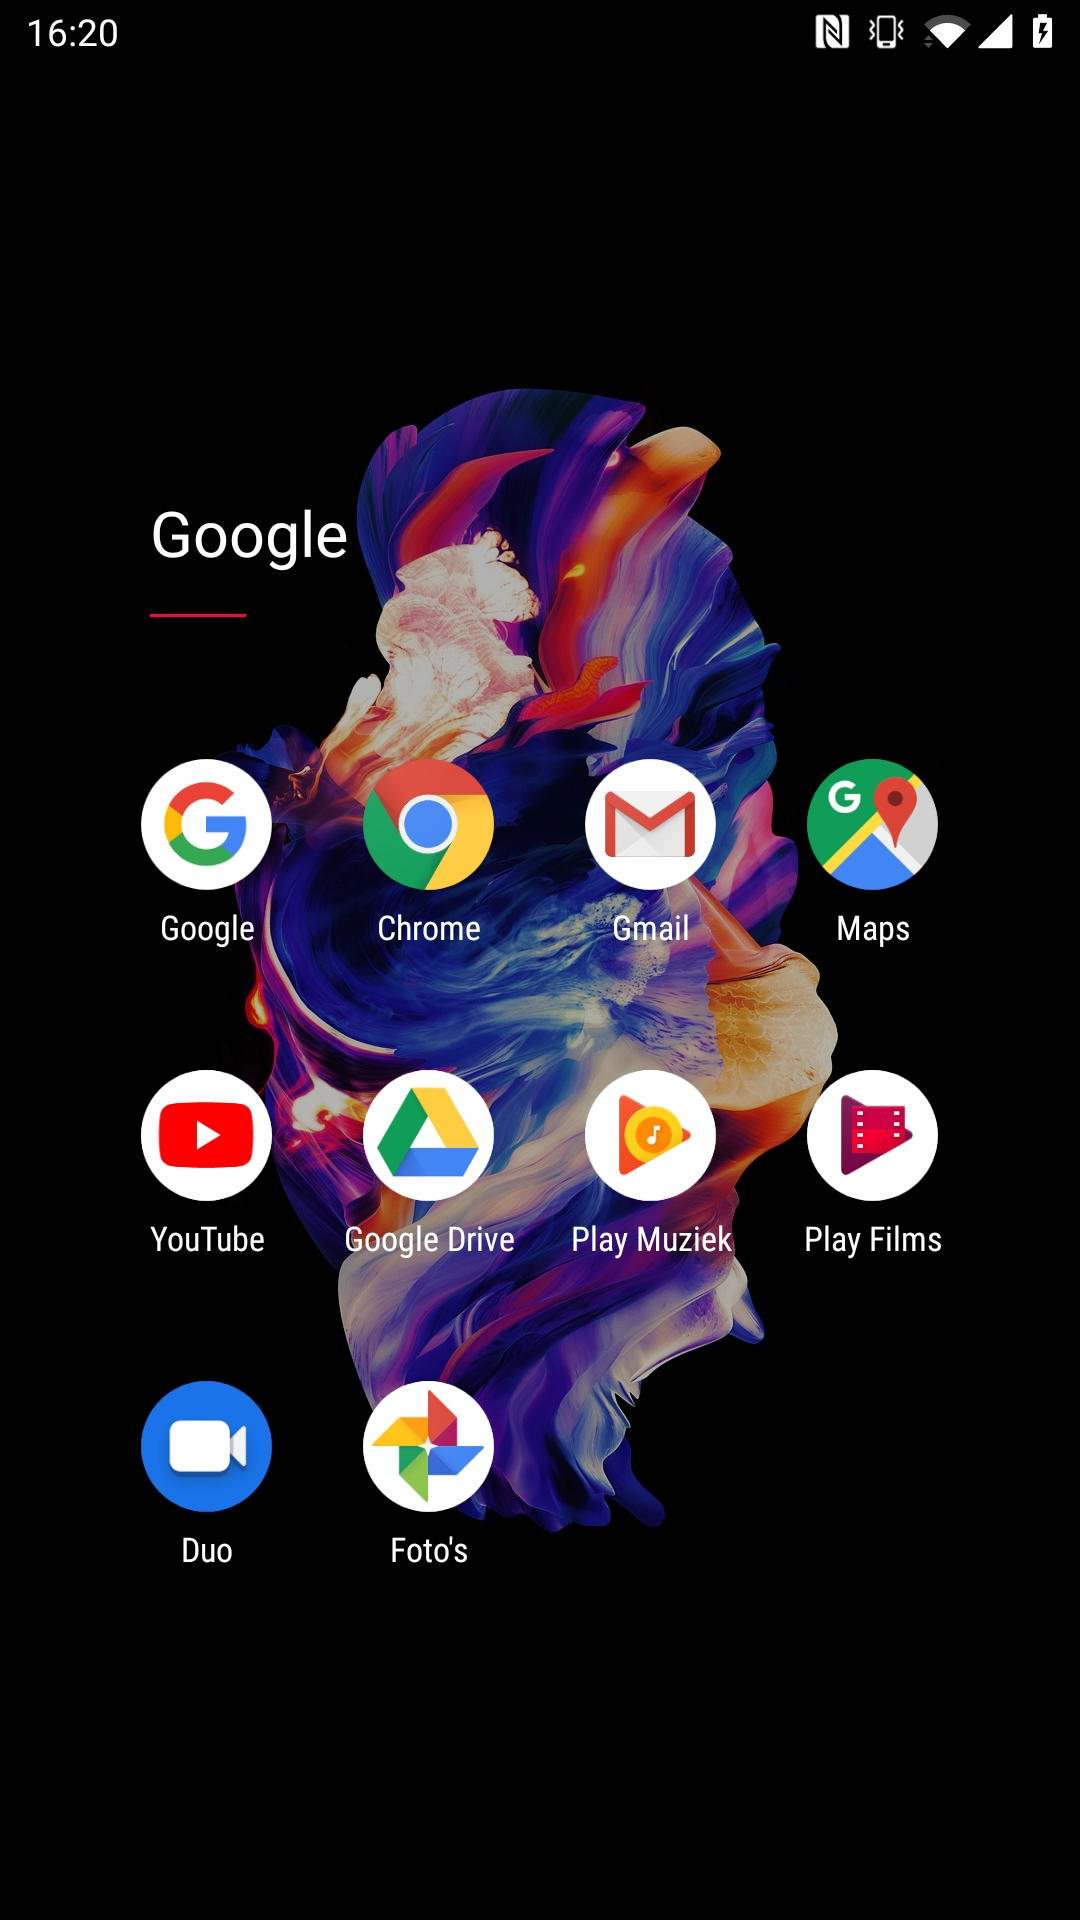
\includegraphics[width=0.4\textwidth]{img/googleapps.jpg}
    \caption{Screenshot van de google applicaties die moeten worden geopend en ingesteld}
    \label{fig:googleapps}
\end{figure}

\subsection{Testgeval 1: Android met fabrieksinstellingen}

Om de toestand van dit testgeval te bekomen, moeten volgende stappen uitgevoerd worden.
\begin{enumerate}
    \item 
    \nameref{itm:factoryreset} (Stap \ref{itm:factoryreset} van terugkerende stappen (\ref{recurringsteps}))
    
    \item 
    \nameref{itm:initialsetup} (Stap \ref{itm:initialsetup} van terugkerende stappen (\ref{recurringsteps}))
    
    \item 
    Stel de Google applicaties in. Ga één voor één door de applicaties in figuur \ref{fig:googleapps} en doorloop  het initiële setup proces. Wanneer er gevraagd wordt om machtigingen te verlenen aan de applicatie, druk dan op toestaan. Open ook de Google Play Store, ga naar 'Mijn apps en games' en druk op 'Alles updaten'.
    
    \item 
    \nameref{itm:developersettings} (Stap \ref{itm:developersettings} van terugkerende stappen (\ref{recurringsteps}))
    
    \item 
    \nameref{itm:disablesleep} (Stap \ref{itm:disablesleep} van terugkerende stappen (\ref{recurringsteps}))
\end{enumerate}


\subsection{Testgeval 2: Android met aangepaste instellingen}

Om de toestand van dit testgeval te bekomen, moeten volgende stappen uitgevoerd worden.

\begin{enumerate}
    \item 
    \nameref{itm:factoryreset} (Stap \ref{itm:factoryreset} van terugkerende stappen (\ref{recurringsteps}))
    
    \item 
    \nameref{itm:initialsetup} (Stap \ref{itm:initialsetup} van terugkerende stappen (\ref{recurringsteps}))
    
    \item Schakel persoonlijke advertenties uit. Navigeer hievoor naar 'Instellingen' > 'Google' > 'Advertenties'. Zet hier 'Afmelden voor personalisatie van advertenties' aan.
    
    \item Stop de data verzameling van locatiegegevens. Dit kan via de webapplicatie van Google gedaan worden of via het apparaat zelf. Om dit te doen via het apparaat zelf, dient men eerst te navigeren naar 'Instellingen' > 'Google' > 'Google account'. Ga dan naar het tabblad 'Gegevens en personalisatie'. Onder de sectie 'Activiteitsopties' moeten 'Web- en app-activiteit' en 'Locatiegeschiedenis' onderbroken worden.
    
    \item Stel een andere DNS-server in. Navigeer hiervoor naar 'Instellingen' > 'Wi-Fi \& internet' > 'Privé-DNS'. Hier kan de gebruiker een DNS-provider naar keuze invullen. Voor dit experiment zal de '1dot1dot1dot1.cloudflare-dns.com' gebruikt worden, een DNS-provider aangeboden door Cloudflare.
    
    \item Stop met het gebruiken van Google applicaties. Hiervoor hoeft er in principe geen extra stap te worden uitgevoerd, maar er kan wel gezorgd worden dat reeds geïnstalleerde Google applicaties niet meer kunnen worden uitgevoerd op de achtergrond. Voor dit experiment zullen de volgende applicaties uitgeschakeld worden: Google Agenda, Google Chrome, Google Contacten, Google Drive, Google Duo, Google Foto's, GBoard, Gmail, Google, Google Play Films, Google Play Muziek, Google Play Store, Google Maps, Youtube. Om dit te doen moet men eerst navigeren naar 'Instellingen' > 'Apps en meldingen' > 'Alle 40 apps bekijken'. Druk één voor één de applicatie aan die u wilt uitschakelen, en druk in het detailscherm op 'uitschakelen'.
    
    \item 
    \nameref{itm:disablesleep} (Stap \ref{itm:disablesleep} van terugkerende stappen (\ref{recurringsteps}))
\end{enumerate}
    
\subsection{Testgeval 3: Aangepaste versie van Android}

Om de toestand van dit testgeval te bekomen, moeten volgende stappen uitgevoerd worden.

\begin{enumerate}
    \item Installeer ADB, Fasboot en Android drivers op een computer. Deze tools geven ons de mogelijkheid om commando's te versturen vanaf onze computer naar de bootloader of herstelmodus van ons apparaat. Een gids voor het installeren van deze tools op verschillende platforms is te vinden op \url{https://www.xda-developers.com/install-adb-windows-macos-linux/}.
    
    \item 
    \nameref{itm:developersettings} (Stap \ref{itm:developersettings} van terugkerende stappen (\ref{recurringsteps}))
    
    \item Schakel USB-foutopsporing in. Deze optie moet ingeschakeld worden zodat een computer kan communiceren met het apparaat via een USB-kabel.
    
    \item Ontgrendel de bootloader van het apparaat. Dit is nodig om een custom ROM te kunnen installeren op het apparaat. Om dit te doen moet OEM-ontgrendeling worden ingeschakeld. Deze optie bevindt zich in 'Instellingen' > 'Systeem' > 'Ontwikkelaarsopties'. Schakel ook 'Geavanceerd herstarten' in. Deze optie laat ons het apparaat makkelijk heropstarten naar de herstelmodus en de bootloader van ons apparaat. Houdt de aan-knop van het apparaat lang in tot er aan de rechterzijde van het scherm opties tevoorschijn komen. Druk hier op 'Bootloader'. Sluit het apparaat aan op de computer met een USB-kabel, en open een terminal venster. Typ hierin 'fastboot oem unlock' en druk op enter. Op het apparaat verschijnt nu een keuzemenu. Selecteer door middel van de volumeknoppen 'Unlock the bootloader' en bevestig met de aan-knop van het apparaat. De bootloader is nu ontgrendeld.
    
    \item 
    Installeer een custom recovery. Deze hebben we nodig om een custom ROM te kunnen installeren. Eerst moeten we hiervoor het '.img' bestand van de custom recovery downloaden. TWRP is de meest gekende custom recovery, aangezien deze heel wat handige functies aanbiedt. Voor dit experiment wordt er gebruik gemaakt van een aangepaste versie hiervan, namelijk TWRP blu\_spark, wegens compatibiliteitsproblemen met het testapparaat. Deze is te vinden op \url{https://github.com/engstk/android_device_oneplus_cheeseburger/releases}. Navigeer in het terminal venster naar de locatie waar dit bestand opgeslagen is, en typ 'fastboot flash recovery lineage-16.0-20190513-microG-cheeseburger.zip'. Hierna kunnen we via de volumeknoppen navigeren naar 'Recovery mode' en deze selecteren door middel van de aan-knop.
    
    \item Nu moet het ROM bestand overgezet worden naar het apparaat. Navigeer naar de locatie waar het ROM bestand zich bevindt en typ 'adb push lineage-16.0-20190513-microG-cheeseburger.zip /data/tmp/lineage.zip'. Het bestand wordt nu overgezet naar het apparaat.
    
    \item Wis het apparaat door binnen TWRP op 'Wipe' te drukken. Selecteer 'Advanced wipe' en klik 'System', 'Data' en 'Cache' aan en bevestig.
    
    \item Installeer de ROM. Druk binnen TWRP op 'Install' en navigeer naar '/data/tmp/'. Selecteer lineage.zip en bevestig de installatie van dit .zip bestand. Eens de installatie voltooid is, druk je op 'Wipe cache/dalvik', en daarna op 'Reboot System'.
    
    \item 
    LineageOS is nu geïnstalleerd! Merk op dat er op het apparaat geen Google applicaties te vinden zijn. De aanwezigheid van microG zorgt ervoor dat applicaties die normaal voortwerken op API's die Google Play Services aanbiedt, nog steeds werken.
    
    \item 
    \nameref{itm:disablesleep} (Stap \ref{itm:disablesleep} van terugkerende stappen (\ref{recurringsteps}))
\end{enumerate}

\section{Monitoring netwerkactiviteit}

\subsection{Testgeval 1: Android met fabrieksinstellingen}

\subsection{Testgeval 2: Android met aangepaste instellingen}

\subsection{Testgeval 3: Aangepaste versie van Android}
Tijdens het uitvoeren van het experiment op testgeval 3 werd er geen data verzameld gedurende alle uitvoeringen van het experiment. Er werd geen enkele netwerkactiviteit gemeten.